\documentclass{article}
\pdfpageheight 21.6cm
\pdfpagewidth 15.15cm
\paperheight 21.6cm
\paperwidth 15.15cm

\usepackage{times}
\usepackage[pdftex]{graphicx}
\usepackage[pdftex]{color}

\voffset 0cm
\textheight 21.6cm

\hoffset 0cm
\oddsidemargin-1.54cm
\evensidemargin-1.54cm
\textwidth 12.85cm

\parindent 0cm

\begin{document}

\pagestyle{empty}

%\definecolor{bcol}{cmyk}{1.000,0.850,0.000,0.000} % background
\definecolor{bcol}{cmyk}{1.00,0,1.000,1.000} % background
\definecolor{tcol}{cmyk}{0.000,0.000,1.000,0.000} % text (title,)
\definecolor{acol}{cmyk}{0.000,0.000,1.000,0.000} % text (, author)
\definecolor{fcol}{cmyk}{0.300,0.255,0.000,0.000} % figure background
\definecolor{scol}{cmyk}{0.000,0.000,0.000,0.000} % text (IMPRS, summary)

\null\vspace{-5cm}

\hspace*{-1.2cm}\colorbox{bcol}{\parbox[b][22cm][c]{15.2cm}{\null\hfill}}

\vspace{-19.4cm}

\hspace*{5mm}\begin{minipage}[t][17.5cm]{12cm}

\begin{center}

\fontencoding{T1}\fontfamily{phv}\fontshape{n}\fontsize{19}{21}\selectfont

\textcolor{tcol}{Observations, analysis and interpretation with non-LTE of chromospheric structures of the Sun}

\vspace{1.8cm}

%\colorbox{fcol}{\parbox[b][62mm][c]{62mm}{\hspace{1mm}

%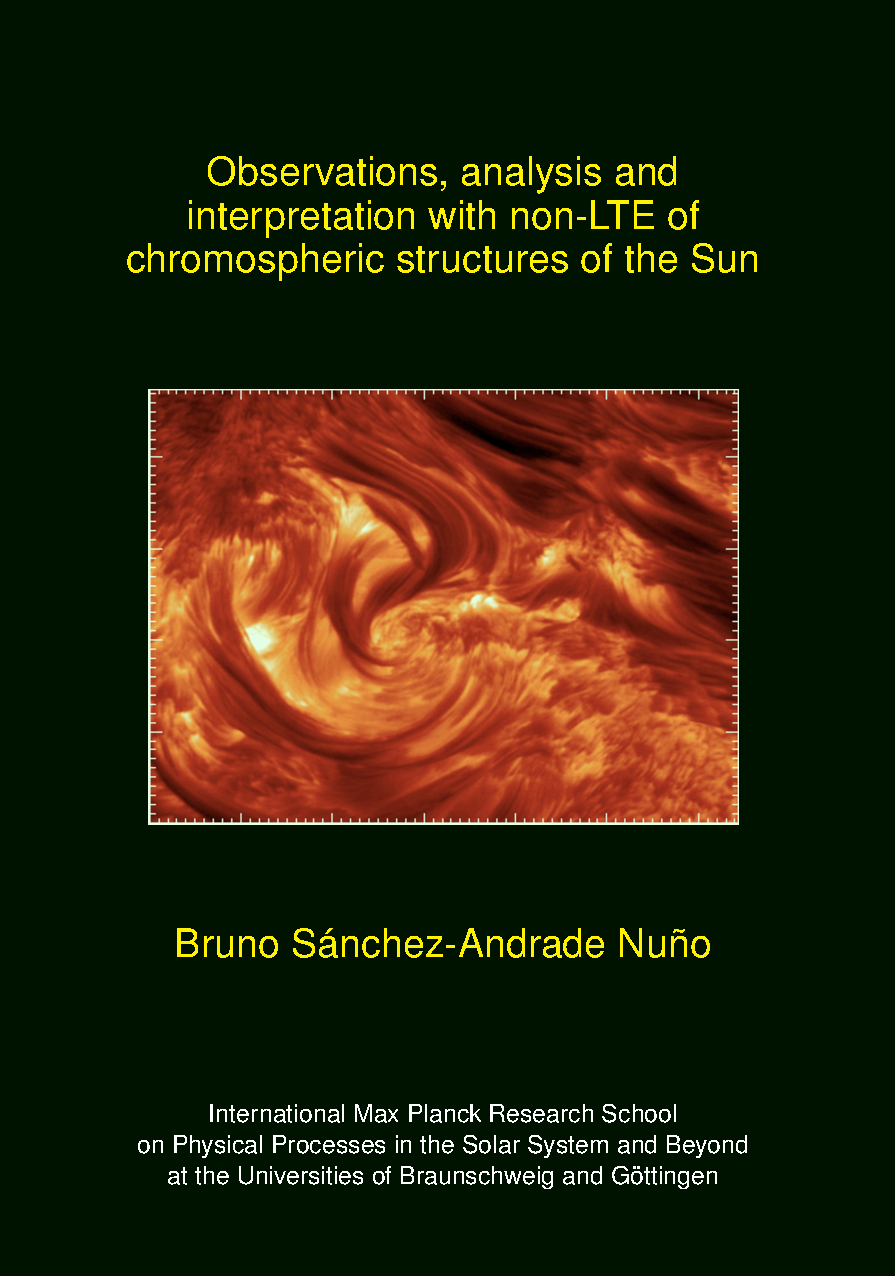
\includegraphics[width=9cm]{../figures/cover.pdf}%}}
%\includegraphics[width=9cm]{../figures/comp-ima-ccd2.pdf}%}}
\includegraphics[width=10cm]{../figures/ha-lc.pdf}%}}


\vspace{1.5cm}

\textcolor{acol}{Bruno S\'anchez-Andrade Nu\~no}

\vfill

\fontencoding{T1}\fontfamily{phv}\fontseries{m}\fontshape{n}\fontsize{12}{15}\selectfont


\textcolor{scol}{International Max Planck Research School\\
on Physical Processes in the Solar System and Beyond\\
at the Universities of Braunschweig and G\"ottingen}

\end{center}

\end{minipage}

\newpage

\null\vspace{-5cm}

\hspace*{-1.2cm}\colorbox{bcol}{\parbox[b][22cm][c]{15.2cm}{\null\hfill}}

\vspace{-19.4cm}

\hspace*{7mm}\begin{minipage}[t][17.5cm]{12cm}

\fontencoding{T1}\fontfamily{phv}\fontshape{n}\fontsize{12}{15}\selectfont

\textcolor{acol}{Bruno S\'anchez-Andrade Nu\~no: Observations, analysis and interpretation with non-LTE of chromospheric structures of the Sun. }

\vspace{0.5cm}

\fontencoding{T1}\fontfamily{phv}\fontseries{m}\fontshape{n}\fontsize{12}{15}\selectfont

\textcolor{scol}{The Sun possesses a complex layer called chromosphere, which extends above the overwhelmingly bright photosphere. With decreasing density, the solar magnetic fields start here to dominate the dynamics, giving rise to new and intricate phenomena. Thus, the chromosphere represents a challenging field of research, from both observational and theoretical aspects.\\
This work comprises the observation of the chromosphere with very high spatial, spectral and temporal resolution. \\ The image analysis, as an important step towards high quality data, is highly involved. We apply various methods and compare the resulting image qualities.\\ The chromosphere is studied both on the solar disc and at the limb. Furthermore, we give interpretations of the observed phenomena by means of current theoretical models.\\
More than a century after its discovery as vividly red rings during total solar eclipses, the chromosphere has remained a paradigm of the marvellous complexity of our Sun.
}

\vfill

\textcolor{scol}{Copernicus GmbH \hfill ISBN 978-3-936586-81-7}

\end{minipage}

\newpage

\null\vspace{-5cm}

\hspace*{-1.2cm}\colorbox{bcol}{\parbox[b][22cm][c]{15.2cm}{\null\hfill}}

\fontencoding{T1}\fontfamily{phv}\fontshape{n}\fontsize{12}{15}\selectfont

\vspace{-21cm}

\hspace*{6cm}\rotatebox{90}{\small \textcolor{tcol}{Bruno S\'anchez-Andrade Nu\~no: \, Observations, analysis and interpretation with non-LTE of chromospheric structures of the Sun}}

\end{document}
